\begin{figure*}[tbp]
  \centering
  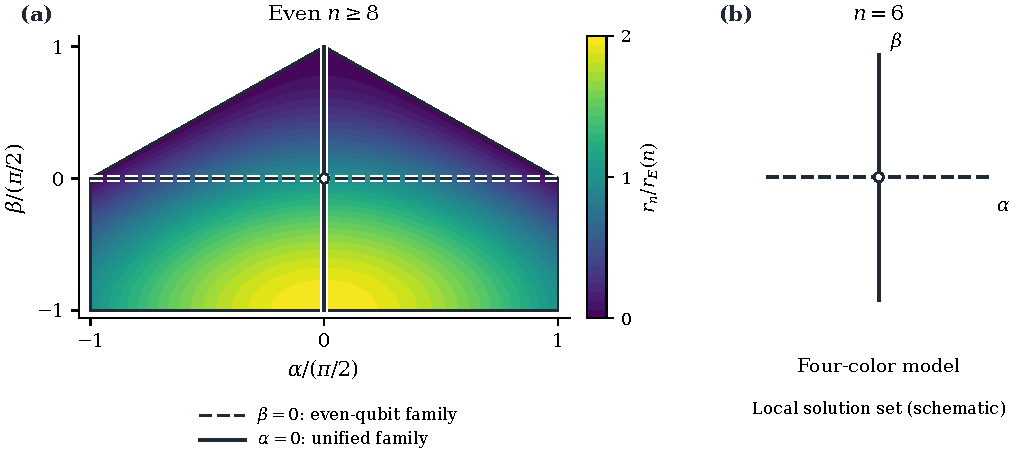
\includegraphics[width=\textwidth]{figures/fig2_embedding.pdf}
  \caption{Two exact sections of an even-qubit two-parameter family.
  (a) For even $n\geq8$, the domain $\Omega$ is given by $|\alpha|\leq\pi/2$ and $-\pi/2\leq\beta\leq\pi/2-|\alpha|$.
  Color represents $r_n/r_E(n)=\cos\alpha-\sin\beta$, with reference radius $r_E(n)=\sqrt3/2^{n-1}$; both axes are in units of $\pi/2$.
  The dashed section $\beta=0$ recovers the prior even-qubit cosine family, and the solid section $\alpha=0$ recovers the unified enhanced family, in each case column by column.
  The open circle marks the common base point.
  (b) Schematic local solution set at $n=6$ in the four-color model, with phases assigned to the four values of $(q_A,q_B)$ and an independent zero-string phase: the two branches cross at the base point.}
  \label{fig:embedding}
\end{figure*}
